%\iffalse
\let\negmedspace\undefined
\let\negthickspace\undefined
\documentclass[journal,12pt,onecolumn]{IEEEtran}
\usepackage{cite}
\usepackage{amsmath,amssymb,amsfonts,amsthm}
\usepackage{algorithmic}
\usepackage{graphicx}
\usepackage{textcomp}
\usepackage{xcolor}
\usepackage{txfonts}
\usepackage{listings}
\usepackage{enumitem}
\usepackage{circuitikz}
\usepackage{mathtools}
\usepackage{gensymb}
\usepackage{comment}
\usepackage[breaklinks=true]{hyperref}
\usepackage{tkz-euclide} 
\usepackage{listings}
\usepackage{gvv}    
\usepackage{enumitem}
\usepackage{amsmath}
\def\inputGnumericTable{}                                 
\usepackage[latin1]{inputenc}                                
\usepackage{color}                                            
\usepackage{array}                                            
\usepackage{longtable}                                       
\usepackage{calc}                                             
\usepackage{multirow}                                         
\usepackage{hhline}                                           
\usepackage{ifthen}                                           
\usepackage{lscape}
\usepackage{tabularx}
\usepackage[italicdiff]{physics}
\usepackage{mathrsfs}
\usetikzlibrary{arrows,positioning}


\newtheorem{theorem}{Theorem}[section]
\newtheorem{problem}{Problem}
\newtheorem{proposition}{Proposition}[section]
\newtheorem{lemma}{Lemma}[section]
\newtheorem{corollary}[theorem]{Corollary}
\newtheorem{example}{Example}[section]
\newtheorem{definition}[problem]{Definition}
\newcommand{\BEQA}{\begin{eqnarray}}
\newcommand{\EEQA}{\end{eqnarray}}
\newcommand{\define}{\stackrel{\triangle}{=}}
\theoremstyle{remark}
\newtheorem{rem}{Remark}
\begin{document}
\bibliographystyle{IEEEtran}
\vspace{3cm}

\title{GATE:2021 - EC 48 }
\author{EE23BTECH11025 - Anantha Krishnan $^{}$% <-this % stops a space
}
\maketitle
\bigskip



\section{question}
A unity feedback system that uses proportional-integral (PI) control is shown in the figure.
 \begin{figure}[!ht]    
    \centering
\graphicspath{ {figs/} }
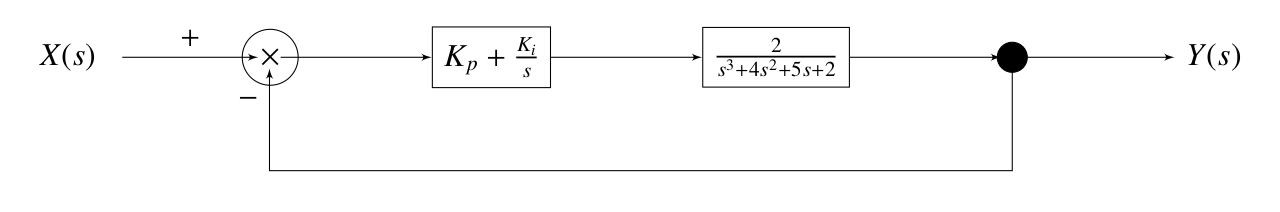
\includegraphics[width=\columnwidth]{figure_1}
\label{figure:ee25-gate4-graph}
\end{figure}
The stability of the overall system is controlled by tuning the PI control parameters $K_p$ and $K_i$. The maximum value of $K_i$ that can be chosen so as to keep the overall system stable or, in the worst case, marginally stable (\textit{rounded off to three decimal places}) is?
\hfill{(GATE EC 2021)}\\
 



\textbf{Solutions :}
%\fi
    
\begin{table}[ht!]
\centering
\begin{tabular}{ |c|c|c| } 
 \hline
Symbols & Description & Values  \\
\hline
$P(s)$ & Plant transfer function & $\frac{2}{s^3+4s^2+5s+2}$ \\
 \hline
 $C(s)$ & PI controller transfer function &$K_p+\frac{K_i}{s}$\\
 \hline
$G(s)$ & Closed loop transfer function &$\frac{P(s)C(s)}{1+P(s)C(s)}$\\
 \hline
$Z$ & Number of zeroes with positive real part in $1+P(s)C(s)$ &?\\
 \hline
 $N$ & Total number of anticlockwise encirclements about $-1+0j$ in Nyquist plot & ?\\
\hline
$P$ & Number of poles with positive real part in $P(s)C(s)$ &?\\
\hline
\end{tabular}
\caption{Parameters, Descriptions, and Values}
\label{table:ee25-ec48-gate2021}
\end{table}




    From table \ref{table:ee25-ec48-gate2021}, the characteristic equation is given as:
    \begin{align}
        1+C(s)P(s) &= 0\\
        1+\brak{K_p+\frac{K_i}{s}}\brak{\frac{2}{s^3+4s^2+5s+2}} &= 0\\
        s^4+4s^3+5s^2+(2+2K_p)s+2K_i &=0 \label{eq:gate 2021 eq:4}
    \end{align}
    For the system to be stable, there must be no sign changes in the first column of the routh array for the above equation. From $\eqref{eq:gate 2021 eq:4}$
    \begin{align}
    \begin{array}{c|cccc}
        s^4 & 1 & 5 & 2K_i \\
        s^3 & 4 & (2 + 2K_p) & 0 \\
        s^2 & \frac{18-2K_p}{4} & 2K_i & 0 \\
        s^1 &  \frac{\brak{\frac{18-2K_p}{4}}\brak{2 + 2K_p}-8K_i}{\frac{18-2K_p}{4}} & 0 & 0\\
        s^0 & 2K_i &0 &0 \\
        \end{array}\\
        \end{align}
        \begin{align}
            \frac{18-2K_p}{4} &> 0\\
            \implies K_p &< 9 \label{eq:gate 2021 eq:1}\\
            \frac{\brak{\frac{18-2K_p}{4}}\brak{2 + 2K_p}-8K_i}{\frac{18-2K_p}{4}} &> 0\label{eq:gate 2021 eq:2}\\
        K_i &>0 \label{eq:gate 2021 eq:3}
    \end{align}
    For marginal stability, assuming 3 cases while maximising $K_i$ and checking if the above inequalities hold.
    \begin{enumerate}
        \item $K_p=9$\\
         \begin{align}
       \brak{\lim_{K_p\to9^-} \frac{\brak{\frac{18-2K_p}{4}}\brak{2 + 2K_p}-8K_i}{\frac{18-2K_p}{4}} > 0} &\cap \brak {K_i > 0}\\
       \brak{\lim_{K_p\to9^-} -8K_i > 0} &\cap \brak{{K_i > 0}}\\
  \implies K_p=9 , \forall K_i &\epsilon (\phi)
    \end{align}
    \item  $K_i=0$\\
    \begin{align}
        \brak{\brak{\frac{18-2K_p}{4}}\brak{2 + 2K_p} > 0}  \cap \brak{K_p < 9}\\
        \implies K_i=0 , \forall K_p \epsilon (-1 , 9)
    \end{align}
    \item $\frac{\brak{\frac{18-2K_p}{4}}\brak{2 + 2K_p}-8K_i}{\frac{18-2K_p}{4}} = 0$\\
        \begin{align}
            \brak{\frac{18-2K_p}{4}}\brak{2 + 2K_p} = 8K_i\\
             -K_p^2 +8K_p + 9 = 8K_i
        \end{align}
        Vertex ($K_p=4$) satisfies $\eqref{eq:gate 2021 eq:1}$:
        \begin{align}
            K_i &= 3.125 \forall (K_p = 4 ,K_i>0)
        \end{align}
    \end{enumerate}

\begin{figure}[!ht]    
    \centering
\graphicspath{ {figs/} }
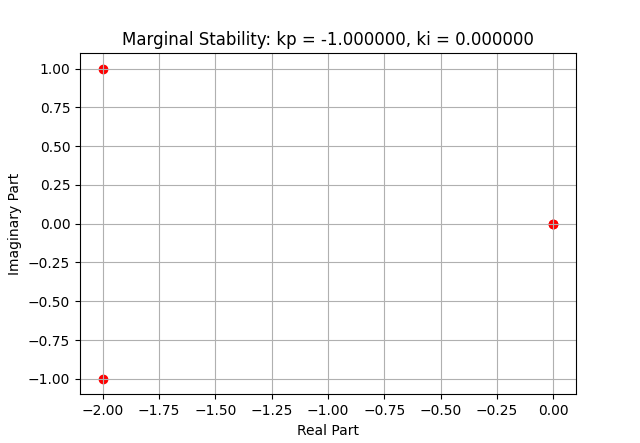
\includegraphics[width=\columnwidth]{graph_1}
\label{figure:ee25-gate4-graph1}
\caption{Location of roots for $k_i=0$,$k_p=-1$}
\end{figure}

\begin{figure}[!ht]    
    \centering
\graphicspath{ {figs/} }
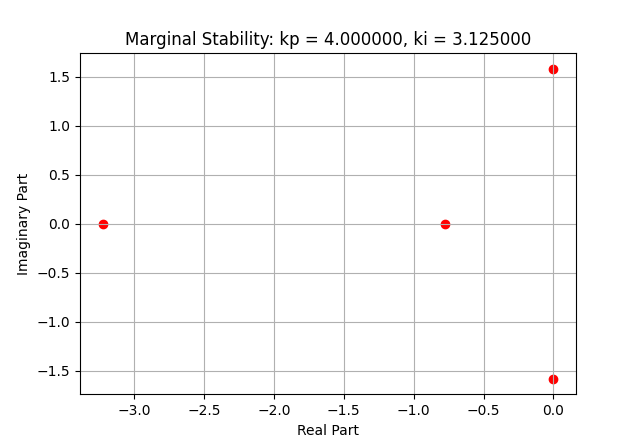
\includegraphics[width=\columnwidth]{graph_2}
\caption{Location of roots for $k_i=0$,$k_p=9$}
\label{figure:ee25-gate4-graph2}
\end{figure}

\begin{figure}[!ht]    
    \centering
\graphicspath{ {figs/} }
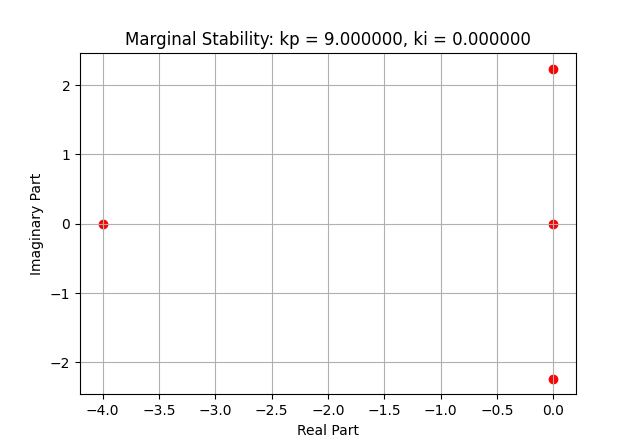
\includegraphics[width=\columnwidth]{graph_3}
\caption{Location of roots for $k_i=3.125$,$k_p=4$}
\label{figure:ee25-gate4-graph3}
\end{figure}
 
    Based on the three cases for marginal stability, the maximum value of $K_i$ is $3.125$, for $K_p = 4$.
   
    
\end{document}


